\chapter{Introduction}\label{ch:intro}

\todo{Should this be optimised for screen or print reading? For example, \LaTeX often places figures with the assumption that a full two-page spread can be seen at one time.}
\todo{Are figure captions included in the word-count? `12,000 words (including tables and footnotes, but excluding appendices, bibliography, photographs and diagrams).'}

\section{Background}\label{sec:intro:background}

In today's fast-moving world of technology, data is king.
The ability to flexibly process large, heterogeneous and asynchronous streams of data is core to many businesses, and this need is only increasing \cite{Yin_2015}\cite{mit_bean_variety}.

Of particular interest are datasets which are inherently unordered and unbounded.
Lack of order arises not just due to clock skew and network latencies.
For instance, consider the issue of tracking play counts of songs on a service like Spotify, where some plays may occur using cached data stored offline, not being sent to the servers until hours later.

Now, suppose we need to aggregate the track play events into user sessions, defined as play events occurring sufficiently close to each other.
The amount of complexity and number of special cases even in this reasonable scenario are too large to consider its implementation as a discrete system.
There is a clear need for an underlying data model and abstraction in order to sanely manage these kinds of computations.

Solutions to this problem have been proposed and implemented in open-source systems such as Apache Storm \cite{apache_storm} and Spark Streaming \cite{spark:zaharia2013discretized}, as well as in company-internal projects like Google's MillWheel \cite{akidau2013millwheel}.
These projects focus on the use of \emph{stream processing}---the assumption that the inputs are (possibly unbounded, or never-ending) streams of data.
They apply techniques such as windowing, triggering and watermark tracking to make processing this kind of data possible, but tend to fall short on sundry features like scalability and fault tolerance, correctness, expressiveness, richness of windowing features, and others.

These solutions are narrowly scoped for particular problem domains, instead of taking a general approach.

\section{Motivation for the Dataflow Model}\label{sec:intro:motivation}

The issues set out in the previous section drove the development of a new, unified model of data processing at Google ~\cite{Akidau:2015}.
This section aims to set out the core motivation behind this model, answering the question, `Why do we need yet another core tool?'

\begin{figure*}[h]
	\centering
	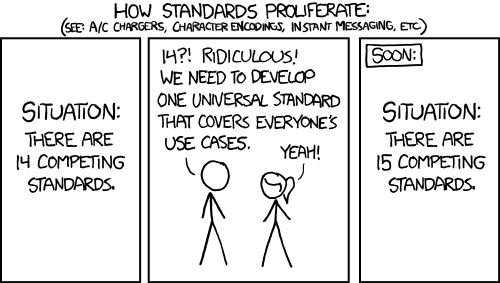
\includegraphics[width=.75\textwidth]{images/xkcd-standards}
	\caption*{\textit{Source: https://xkcd.com/927/\quad(CC BY-NC 2.5)}}
\end{figure*}

Simply put, the Dataflow Model aims to provide a unified way of thinking about stream- and batch-oriented processing, resulting in a composable abstraction of computation.
It acknowledges the fact that it is impossible to design a perfect (always correct, low-latency and cheap) system, and instead it allows for tunability across these characteristics.

\Cref{sec:prep:dataflow} dives deep into the Model itself and explains how these aims are achieved, while \cref{ch:impl} contains a detailed overview of the implementation of the Model in practice.

\section{Why Elixir?}\label{sec:intro:elixir}

The Elixir language \cite{Elixir} is relatively young.
It is currently most popular in the web development circles, with many treating it as a Ruby replacement.
How then is it a suitable language in which to implement a robust, complex data processing system?

The answer lies in the underpinnings of the language.
Beneath the shiny, modern exterior lie the battle-hardened BEAM Virtual Machine (VM) and the OTP framework, which have powered Erlang systems in mission-critical industries like telecoms for decades.
We also have at our disposal the entire ecosystem of libraries written for Erlang.

Elixir is a dynamically typed, functional language with no variable mutability. 
It executes on the BEAM VM which can efficiently manage and schedule hundreds of thousands of \emph{processes}---small user-space threads.
This invites the use of an actor-based model for applications, and indeed this is the standard approach in the Elixir/BEAM ecosystem.

These built-in primitives allow us to closely implement the desired semantics of the Dataflow Model without the overhead of thousands of lines of scheduling, threading and co\"ordinating\footnotemark[1] code (present in the existing Java implementation).

\footnotetext[1]{
For the typographically observant reader: the \"{} mark in ``co\"ordinating'' is a diaeresis---one of the two diacritical marks which are part of English natively (the other being the grave, as in ``the learn\`ed scholar'').
While its use is uncommon in modern English, some publications (notably The New Yorker) still employ it, and including it is the preferred style of the author.
It is used to indicate that two vowels should be pronounced separately, and not as a diphthong.
}

This project was completed using Elixir v1.4.2, and so all code examples and statements about the language apply to this version, the most current at the time of writing.

\Cref{sec:prep:elixir} gives a brief introduction to the language syntax and semantics.



\section{Previous work}\label{sec:intro:previous}
Since the publication of the Dataflow paper in 2015 \cite{Akidau:2015}, work has been ongoing to implement the Model in practice.
Initially, Google released the Google Cloud Dataflow product \cite{CloudDataflow} along with an SDK to allow users to construct data processing pipelines and run them on Google's cloud infrastructure.

In early 2016, Google decided to open-source the project and place it under the care of the Apache Foundation \cite{ApacheDataflowPost}.
This marked the beginning of Apache Beam, a project whose goals were even wider, and include support for cross-platform, cross-language compatibility through separating the creation of the pipelines and their execution on \emph{runners}.

The project has made excellent progress on these fronts, with a fully-featured SDK written in Java as well as a Python SDK.
Its pipelines can be executed on many systems including the Apache projects Spark, Storm and Flink.
Google Cloud Dataflow remains a paid product capable of running Beam pipelines at scale, but is now only one of many options for doing so.

Important to mention is an attempt to bring some of the ideas in the Dataflow Model to an idiomatic Elixir-only library, Flow \cite{ElixirFlow}.
This drove the development of GenStage \cite{ElixirGenStage}, a low-level library implementing demand-driven data flow between actor processes, along with an extensible way to route, partition and dispatch that data.
The GenStage library forms the backbone of the execution logic in this project, and it is discuessed in \cref{sec:impl:approach:genstage}.

\section{Terminology}\label{sec:intro:terminology}

There are several similar and overloaded terms employed in this dissertation.
This section aims to clarify these and set a convention to be followed.
For a full list of defined terms, the reader should consult the glossary in \cref{apx:glossary}.

Due to the naming change to Apache Beam on open-sourcing the project, various references to both `Dataflow` and `Beam` can be found on the web with little consistency.

The approach taken in this paper is to refer to the theoretical model proposed by Akidau et al.\ \cite{Akidau:2015} as the Dataflow Model, and to the current, \emph{de facto} official, implementation \cite{ApacheBeam} as Beam.
Further, where the `Beam Model' is referenced, the author means the Dataflow extended with concepts now found in Apache Beam.
These concepts are described in detail in \cref{sec:impl:dataflow}.

The virtual machine which powers Erlang and Elixir is called the BEAM.
In this unfortunate case of overloading, the Apache project will be referred to as Beam, with all-uppercase BEAM being reserved for the virtual machine.

\section{Goals and focus}\label{sec:intro:goals}

At the outset, the goal of the project was to write an Elixir-based SDK able to create Pipelines compatible with existing Beam software.
Several weeks into the research it emerged both that this approach was impractical to achieve, and that the front-end DSL itself was a relatively small task in itself, not suitable to form the entirety of the project.

The goal then shifted to writing an implementation of a subset of the Beam Model in Elixir.
However, due to the lack of explicit technical documentation of the Model, it quickly became clear that in order to achieve this, a significant amount of work had to be done to reverse-engineer it from an existing open-source codebase and community discussions.
As explained in \cref{sec:impl:dataflow}, many concepts have to be introduced in order to implement the Model, but they are not described directly in any reference material.

Therefore, a second goal of the project emerged, which proved to be a major focus---to extend and clarify the Dataflow Model with the concepts found in Apache Beam, such that a fuller, implementation-ready description is produced.
Once this work was completed, the initial goal of implementing a subset of this extended model was achieved with some additional effort.

\section{Results achieved}\label{sec:intro:results}

Overall, the project was a success, in spite of proving much more challenging than originally expected.
Due to the highly uncertain nature of the requirements which were discovered incermentally as the project progressed, code had to be continually revisited and improved upon, and evaluation of progress was not straightforward.

Nevertheless, a working implementation of the Model was produced.
The implementation, while forgoing some features, delivered robust performance and a clean programmer interface, meshing well with existing language conventions.

A significant amount of currently non-existent documentation of the theory of the Beam Model was also produced, with some further extensions introduced which solve problems currently being tackled in the Beam Project.

